\documentclass[10pt,a4paper]{article}
\usepackage[T1]{fontenc}
\usepackage[utf8]{inputenc}
\usepackage{mathpazo}
\usepackage{microtype}
\usepackage[margin=1.85cm,top=1.7cm,bottom=1.7cm]{geometry}
\usepackage{needspace,booktabs,graphicx,xcolor,caption,array,multirow,enumitem,titlesec,float}
\usepackage{tikz,pgfplots}
\pgfplotsset{compat=1.17}
\usetikzlibrary{arrows.meta,positioning}
\usepackage[hidelinks]{hyperref}

\definecolor{ink}{HTML}{1B1A17}
\definecolor{brick}{HTML}{A23B2A}
\definecolor{olive}{HTML}{5E6B2D}
\definecolor{ochre}{HTML}{B07A1E}
\definecolor{ash}{HTML}{9C968A}
\definecolor{paper}{HTML}{EFEAE0}

\captionsetup{font=small,labelfont=bf,skip=3pt}
\titleformat{\section}{\large\bfseries}{\thesection}{0.6em}{}
\titleformat{\subsection}{\normalsize\bfseries\itshape}{\thesubsection}{0.5em}{}
\titlespacing*{\section}{0pt}{9pt}{3pt}
\titlespacing*{\subsection}{0pt}{6pt}{2pt}
\setlength{\parskip}{3pt}\setlength{\parindent}{0pt}
\setlist{nosep,leftmargin=1.3em}
\renewcommand{\arraystretch}{1.12}
\pgfplotsset{every axis/.append style={font=\footnotesize,tick label style={font=\scriptsize},label style={font=\scriptsize},legend style={font=\scriptsize,draw=none,fill=none},axis line style={ink},grid style={ash!35}}}

\newcommand{\figimg}[2]{\includegraphics[#1]{#2}}

\begin{document}

\thispagestyle{empty}\pagenumbering{gobble}
{\fontsize{30}{34}\selectfont\bfseries SplitSnap}\\[3pt]
{\Large Reading a restaurant bill from a photo, and splitting it fairly}\\[3pt]
{\large Model report \quad Nalafaad Hackathon, Track 1}
\vspace{5pt}\hrule\vspace{9pt}

\subsection*{The problem}
Every group meal ends with a crumpled bill and an argument about who owes what. The sums are easy. Reading the bill correctly, and dividing it in a way each person would call fair, is not: shared dishes, someone who only had a drink, a service charge, a discount, a rounding line, two kinds of GST.

\subsection*{What we built}
SplitSnap takes one photo of the bill and reads it with a model we trained ourselves. The user then fixes whatever was misread, names the people at the table, says who had what, and gets an exact split. Every tax, service charge, packaging fee, discount and rounding line is shared in proportion to what each person ordered, never equally, and each person receives a short written account of how their amount was reached. A person's amount can be overridden by hand, and an override is marked as such.

\subsection*{How to read the evidence}
Accuracy on CORD and SROIE is measured on their held-out test splits. We did not have photographed Indian bills, so everything we say about Indian-style layouts comes from bills our own generator draws, and the report labels those results that way each time. Section~\ref{sec:limits} says what that does and does not show.

\subsection*{Requirements and where this report covers them}
\begingroup\footnotesize
\begin{tabular}{@{}lp{10.6cm}l@{}}
\toprule
 & What the report shows & Section\\
\midrule
R1 & Donut fine-tuned by us on CORD, SROIE and generated bills; scores before and after training on bills not seen anywhere & \ref{sec:ft}, \ref{sec:res}\\
R2 & Confidence per field, the doubtful 8\% highlighted, retake prompt for poor photos; tested on CORD and generated bills, not on real faded or blurred photos & \ref{sec:charges}, \ref{sec:app}\\
R3 & Every item, price, quantity and charge editable; totals recomputed live; corrections flow into the split & \ref{sec:app}\\
R4 & No closed or paid model or API anywhere in the pipeline & end of \ref{sec:limits}\\
R5 & Eleven charge types shown on separate lines and divided per person & \ref{sec:charges}\\
R6 & A written explanation for every person, from the same numbers as the split & \ref{sec:charges}, \ref{sec:app}\\
R7 & Any person's amount can be overridden; the result is stamped as adjusted by hand & \ref{sec:app}\\
R8 & Any number of named people, changeable at any point & \ref{sec:app}\\
\bottomrule
\end{tabular}
\endgroup

\vspace{2pt}
\setcounter{tocdepth}{1}
\renewcommand{\contentsname}{Contents}
{\footnotesize\setlength{\parskip}{0pt}\tableofcontents}
\clearpage\pagenumbering{arabic}\setcounter{page}{1}

\textbf{Summary.}
SplitSnap takes one photo of a restaurant or canteen bill, extracts the items and charges with a model we fine-tuned ourselves, lets the user correct whatever was misread, and divides the bill among named people. Taxes, service charge, packaging, discounts and rounding are shared in proportion to what each person ordered, not equally, and every person gets a plain-language account of their amount. The extractor is Donut (\texttt{naver-clova-ix/donut-base}, 202 M parameters), fine-tuned on CORD, SROIE and generated Indian-style bills. On the held-out test splits it reaches a field F1 of 0.894 on CORD (95 bills) and 0.872 on SROIE (347 bills), and it reads a bill in a median of 0.455\,s on a Kaggle T4. We had no photographed Indian bills, so behaviour on Indian-style layouts is measured on generated bills; Section~\ref{sec:limits} says what that does and does not show.

\section{The system}\label{sec:sys}
Figure~\ref{fig:pipe} shows the path of one bill. Only the second box is a learned model; the arithmetic after it is exact (integer paise), so any error in the final amounts traces back to a visible, editable field. Nothing in the pipeline calls an external service: the model runs on local weights and the web app is a FastAPI server with a plain JavaScript front end.

\begin{figure}[!ht]
\centering
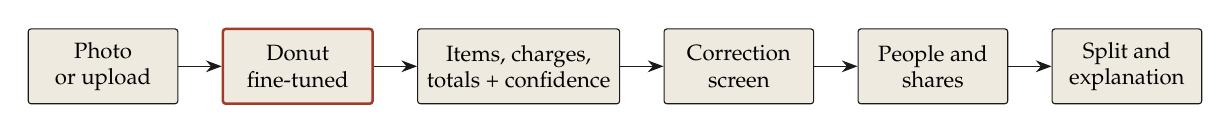
\begin{tikzpicture}[node distance=5.5mm,every node/.style={font=\footnotesize},
 box/.style={draw=ink,rounded corners=1pt,minimum height=9.5mm,minimum width=19mm,align=center,fill=paper},
 hl/.style={draw=brick,line width=0.9pt,rounded corners=1pt,minimum height=9.5mm,minimum width=19mm,align=center,fill=paper},
 arr/.style={-{Stealth[length=2mm]},ink}]
\node[box](a){Photo\\or upload};
\node[hl,right=of a](b){Donut\\fine-tuned};
\node[box,right=of b](c){Items, charges,\\totals + confidence};
\node[box,right=of c](d){Correction\\screen};
\node[box,right=of d](e){People and\\shares};
\node[box,right=of e](f){Split and\\explanation};
\foreach \x/\y in {a/b,b/c,c/d,d/e,e/f}{\draw[arr](\x)--(\y);}
\end{tikzpicture}
\caption{The path of one bill. The red box is the model we trained; every box after it is deterministic code that is unit tested.}\label{fig:pipe}
\end{figure}

\section{Base model}\label{sec:base}
We started from \texttt{naver-clova-ix/donut-base}, an OCR-free encoder--decoder (Swin encoder, BART-style decoder) that reads the image and writes a token sequence directly. Three practical points decided it. It needs no separate text-recognition stage, so there is one model to train and one place to look when a field is wrong. At 202 M parameters it can be fully fine-tuned on one 16 GB T4 at 1280$\times$960 input (7.8 GB peak). And the probabilities of the tokens it writes give a per-field confidence at no extra cost, which the correction screen uses to highlight doubtful fields.

We also ran several open vision-language models zero-shot on the same 20 CORD bills (Table~\ref{tab:zs}). This was done to see what a larger model could do before any training, not to pick the winner: the public CORD-trained Donut leads on CORD because it was trained on CORD's labelling conventions, and the Qwen models are well behind it on those conventions but far slower. We did not fine-tune any of the vision-language models, so we cannot say how they would compare with our Donut after training; we chose Donut for its speed (Section~\ref{sec:opt}), its fit to the free-tier compute budget and its built-in confidence.

\begin{table}[!ht]
\centering\small
\begin{tabular}{@{}lrrr@{}}
\toprule
Model (Kaggle T4, fp16) & CORD field F1 & s per bill & GPU memory (GB)\\
\midrule
Donut-base, pretrained only, not fine-tuned (our starting point; 6 bills) & 0.00 & n/a & n/a\\
Donut, public CORD-trained by its authors (not ours) & 0.91 & 0.6 & n/a\\
Qwen3-VL-2B-Instruct & 0.73 & 10.6 & 4.6\\
Qwen3-VL-4B-Instruct & 0.66 & 10.3 & 9.4\\
Qwen2.5-VL-3B-Instruct & 0.61 & 13.3 & 7.8\\
Qwen2-VL-2B-Instruct & 0.45 & 15.2 & 4.8\\
\midrule
Ours, fine-tuned Donut (all 95 CORD test bills, a different sample) & 0.894 & 0.455 & 0.72\\
\bottomrule
\end{tabular}
\caption{Field F1 on CORD test bills (our own metric code). Rows 2 to 6 are zero-shot on the same 20 bills, where one bill is five points; the public CORD-trained Donut had already been trained on CORD by its authors. The last row is our fine-tuned model on the full CORD test split, so it is not a controlled comparison; times for it are from the T4 (0.455 s) and GPU memory from the laptop (0.72 GB).}\label{tab:zs}
\end{table}

\section{Data and splits}\label{sec:data}
\textbf{CORD} (Indonesian receipts) was converted to our schema: a list of items with name, quantity, unit price and total, a list of typed charges, a subtotal and a grand total. \textbf{SROIE} (Malaysian scans) has only four labelled fields per receipt (company, date, address, total), so it is trained as a second task behind its own start token. Because both datasets are retail receipts without GST lines, we added \textbf{generated Indian-style bills}: our generator (\texttt{splitsnap/synth.py}) draws restaurant and mess bills with CGST, SGST, GST, service charge, packaging, discounts and round-off in many wordings, with whole-rupee and decimal prices, up to nine font families and thermal-print fading. The labels are exact by construction. These are whole generated bills and not light augmentation, so we report them separately and never count them as real-bill evidence.

\begin{table}[!ht]
\centering\small
\begin{tabular}{@{}lrrrl@{}}
\toprule
Source & Train & Validation & Test & Notes\\
\midrule
CORD & 769 & 98 & 95 & official splits, unusable records and outliers dropped\\
SROIE & 558 & 59 & 347 & official test split; 60 train scans held out\\
Generated Indian-style bills & 700 & 100 & 100 & seeds fixed; labels exact\\
\bottomrule
\end{tabular}
\caption{Splits. A manifest check confirmed that no image appears in more than one split; eight byte-identical SROIE images that the official split had placed in two splits were removed from the less protected one.}
\end{table}

The checkpoint was chosen on validation bills only (mean of the CORD edit-distance score and the SROIE field score); the test splits were used once, after training.

\begin{figure}[!ht]
\centering
\figimg{height=3.3cm}{../examples/sroie/sroie_test_X00016469670.jpg}\hfill
\figimg{height=3.3cm}{../examples/sroie/sroie_test_X51005200931.jpg}\hfill
\figimg{height=3.3cm}{../examples/sroie/sroie_test_X51005230605.jpg}\hfill
\figimg{height=3.3cm}{../examples/sroie/sroie_test_X51005230616.jpg}\\[3pt]
\figimg{height=2.9cm}{../examples/synthetic_flat/synth_1.png}\hfill
\figimg{height=2.9cm}{../examples/synthetic_flat/synth_2.png}\hfill
\figimg{height=2.9cm}{../examples/synthetic_flat/synth_3.png}
\caption{Top: four SROIE test scans (handwritten totals and stamps are common). Bottom: three generated Indian-style bills as the generator draws them, before any photo effects.}\label{fig:data}
\end{figure}

\subsection{Augmentation}
Training images are altered on the fly with a profile per source. All profiles use small rotation ($\pm 6^\circ$) and perspective, blur, brightness and contrast changes, JPEG compression and lower-resolution capture. The SROIE and generated profiles add a table, cloth or wood background with a thin margin, a contact shadow, creases, paper curl, vignetting and a colour cast; the CORD profile is gentler because those photos are already soft. Validation and test bills from the generator get one fixed realistic augmentation so that their scores are repeatable.

\begin{figure}[!ht]
\centering
\figimg{height=2.9cm}{../examples/augmentation_by_profile/synth_original.jpg}\hfill
\figimg{height=2.9cm}{../examples/augmentation_by_profile/synth_profile_example_0.jpg}\hfill
\figimg{height=2.9cm}{../examples/augmentation_by_profile/synth_profile_example_1.jpg}\hfill
\figimg{height=2.9cm}{../examples/augmentation_by_profile/synth_profile_example_2.jpg}\\[3pt]
\figimg{height=3.5cm}{../examples/augmentation_by_profile/sroie_original.jpg}\hfill
\figimg{height=3.5cm}{../examples/augmentation_by_profile/sroie_profile_example_0.jpg}\hfill
\figimg{height=3.5cm}{../examples/augmentation_by_profile/sroie_profile_example_1.jpg}\hfill
\figimg{height=3.5cm}{../examples/augmentation_by_profile/sroie_profile_example_2.jpg}
\caption{Augmentation. Left of each row: the original; to the right, three random draws from that source's profile.}\label{fig:aug}
\end{figure}

\section{Fine-tuning}\label{sec:ft}
The target for each bill is serialised in the Donut way, as a token sequence with an opening and closing token for each field (item name, quantity, unit price, total; charge type and amount; subtotal; grand total), and the decoder is trained to produce it from the image. The longest target in the data is 444 tokens, so the limit is 512. Table~\ref{tab:hp} lists the setup; both Kaggle sessions used the same 16-epoch cosine schedule, and the second resumed from the first one's checkpoint, optimiser and scheduler state.

\begin{table}[!ht]
\centering\small
\begin{tabular}{@{}ll@{\hspace{2em}}ll@{}}
\toprule
Initialisation & \texttt{donut-base} + our tokens & Epochs & 16 (2,027 samples each)\\
Input size & 1280$\times$960 & Optimiser & AdamW (fused), lr $3\times10^{-5}$, cosine\\
Precision & fp16 mixed, fp32 master weights & Warm-up & 10\% of steps\\
Batch & 1 $\times$ 8 accumulation & Speed & 0.42 s per sample, 13.9 min per epoch\\
Trainable & all 202 M parameters & Peak GPU memory & 7.8 GB (T4, 16 GB)\\
Hardware & Kaggle T4 & Total & 2 sessions, 126 + 119 min\\
\bottomrule
\end{tabular}
\caption{Fine-tuning setup.}\label{tab:hp}
\end{table}

\begin{figure}[!ht]
\centering
\begin{tikzpicture}
\begin{axis}[width=0.47\textwidth,height=4.6cm,ymode=log,xlabel={epoch},ylabel={training loss},xmin=1,xmax=16,grid=major,title={\footnotesize Training loss}]
\addplot[brick,thick,mark=*,mark size=1.3pt] table[x=x,y=y]{data/loss.dat};
\end{axis}
\end{tikzpicture}\hfill
\begin{tikzpicture}
\begin{axis}[width=0.47\textwidth,height=4.6cm,xlabel={epoch},ylabel={validation score},xmin=3,xmax=17,ymin=0.8,ymax=1.0,grid=major,title={\footnotesize Validation score (higher is better)},legend pos=south east,legend columns=1]
\addplot[ink,thick,mark=square*,mark size=1.3pt] table[x=x,y=y]{data/val_cord.dat}; \addlegendentry{CORD edit-distance score}
\addplot[brick,thick,dashed,mark=*,mark size=1.3pt] table[x=x,y=y]{data/val_sroie.dat}; \addlegendentry{SROIE field score}
\addplot[olive,thick,dotted,mark=triangle*,mark size=1.5pt] table[x=x,y=y]{data/val_synth.dat}; \addlegendentry{Generated bills}
\end{axis}
\end{tikzpicture}
\caption{Left: training loss per epoch (log scale). Right: validation scores every second epoch from epoch 4, on 25 CORD, 25 SROIE and 10 generated validation bills. The checkpoint at epoch 16 was kept.}\label{fig:curves}
\end{figure}

\section{Results}\label{sec:res}
\subsection{Held-out test splits}
Table~\ref{tab:test} gives the scores on the test splits, computed with our own implementation of the metrics (\texttt{metrics.py}): tree edit distance accuracy (TED), precision, recall and F1 over (field, value) pairs, and exact match for the four SROIE fields. On CORD, the public CORD-trained Donut scored a field F1 of 0.90 on a 30-bill subset; ours scores 0.894 on all 95 test bills, so the two are close but come from different bill sets and are not a controlled comparison. The generated-bill scores are high because the model is reading the same generator it trained on; they are shown for completeness, not as evidence about real bills.

\begin{table}[!ht]
\centering\small
\begin{tabular}{@{}lrl@{}}
\toprule
Test set (n) & & Scores\\
\midrule
CORD (95) & & TED 0.930; field precision / recall / F1 0.896 / 0.893 / 0.894; item F1 0.876;\\
 & & charge F1 0.800; subtotal correct 94.7\%; grand total correct 94.7\%\\
SROIE (347) & & exact match: company 85.3\%, date 95.1\%, address 78.4\%, total 87.3\%; micro F1 0.872\\
Generated Indian-style (100) & & TED 0.997; field F1 0.985; item F1 0.997; charge F1 0.972; grand total 98\%\\
\bottomrule
\end{tabular}
\caption{Held-out test results, epoch-16 checkpoint.}\label{tab:test}
\end{table}

\begin{figure}[!ht]
\centering
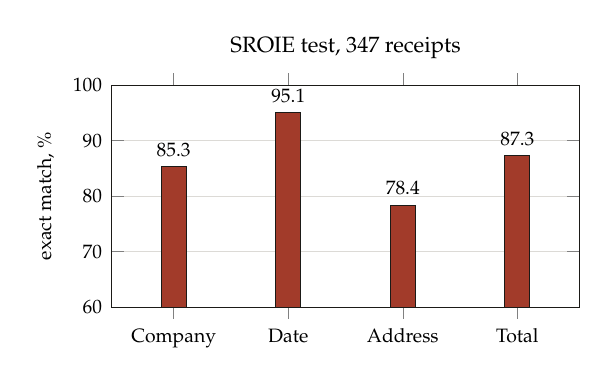
\begin{tikzpicture}
\begin{axis}[ybar,width=0.62\textwidth,height=4.4cm,bar width=9pt,symbolic x coords={Company,Date,Address,Total},xtick=data,ymin=60,ymax=100,ylabel={exact match, \%},nodes near coords,every node near coord/.append style={font=\scriptsize},enlarge x limits=0.18,title={\footnotesize SROIE test, 347 receipts},ymajorgrids]
\addplot[fill=brick,draw=ink] coordinates {(Company,85.3) (Date,95.1) (Address,78.4) (Total,87.3)};
\end{axis}
\end{tikzpicture}\hfill
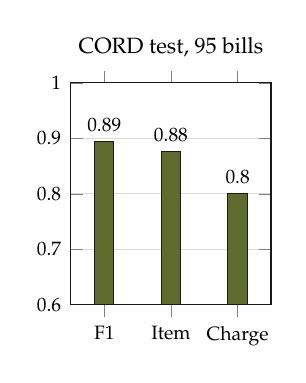
\begin{tikzpicture}
\begin{axis}[ybar,width=0.34\textwidth,height=4.4cm,bar width=7pt,symbolic x coords={F1,Item,Charge},xtick=data,ymin=0.6,ymax=1.0,nodes near coords,every node near coord/.append style={font=\scriptsize},enlarge x limits=0.25,title={\footnotesize CORD test, 95 bills},ymajorgrids]
\addplot[fill=olive,draw=ink] coordinates {(F1,0.894) (Item,0.876) (Charge,0.800)};
\end{axis}
\end{tikzpicture}
\caption{Test scores by field.}\label{fig:testbars}
\end{figure}

\subsection{Before and after fine-tuning on new Indian-style bills}
To show the effect of training directly, we made 100 further generated bills with seeds that no earlier step used (Figure~\ref{fig:newbills}) and ran the first 30 of them through two models with the same decoding settings: \texttt{donut-base} with its original pretrained weights (it was trained to read text in general, never on receipts or on our output format), plus our added tokens and input size, and the fine-tuned model. These bills were never seen in training, validation or test. The pretrained model has never seen our tags or start token: on the first two bills its raw output is the start token followed at once by the end token (two tokens, no items), where the fine-tuned model writes about 150 tokens of items, so with nothing predicted every field-level score is zero and the edit-distance score is small but not zero, since an empty bill still shares part of the target's skeleton (Table~\ref{tab:ba}); after fine-tuning, all 30 grand totals and subtotals are right and the field F1 is 0.988. The one wrong field in the first bill is shown in Figure~\ref{fig:newbills}.

\begin{figure}[!ht]
\centering
\figimg{height=3.0cm}{../examples/final_run/final_001.jpg}\hfill
\figimg{height=3.0cm}{../examples/final_run/final_002.jpg}\hfill
\figimg{height=3.0cm}{../examples/final_run/final_003.jpg}\hfill
\figimg{height=3.0cm}{../examples/final_run/final_004.jpg}\hfill
\figimg{height=3.0cm}{../examples/final_run/final_005.jpg}\\[4pt]
{\footnotesize\begin{tabular}{@{}lp{12.9cm}@{}}
\toprule
Bill 1 (left photo) & \\
\midrule
Label & Dal Tadka, Egg Curry, Veg Sandwich, Filter Coffee, Samosa, Mutton Curry; Discount $-$181.65, Service charge 60.55, CGST 61.76, SGST 61.76; total 1213.42\\
Not fine-tuned & nothing: an empty bill, no items, no charges, no totals\\
Fine-tuned model & the same six items and four charges, subtotal 1211, total 1213.42; Mutton Curry unit price read as \textcolor{brick}{310} where the label says 305 (its line total, 610, is right)\\
\bottomrule
\end{tabular}}
\caption{Five of the new bills, and what the two models produced for the first. The mistake is the kind the correction screen is for: a digit in a unit price, with the line total correct.}\label{fig:newbills}
\end{figure}

\begin{table}[!ht]
\centering\small
\begin{tabular}{@{}lrr@{}}
\toprule
Measure & Before (not fine-tuned) & After (fine-tuned)\\
\midrule
TED accuracy & 0.065 & 0.998 \\
Field F1 & 0.000 & 0.988 \\
Item F1 & 0.000 & 1.000 \\
Charge F1 & 0.000 & 0.964 \\
Grand total correct & 0.000 & 1.000 \\
Subtotal correct & 0.000 & 1.000 \\
Passes arithmetic check & 0.000 & 1.000 \\
\bottomrule
\end{tabular}

\caption{Before and after fine-tuning on bills not used anywhere in training or selection.}\label{tab:ba}
\end{table}


\subsection{Robustness to poor photos}
The 100 unseen generated bills were degraded in controlled steps (Gaussian blur of 1.5, 3 and 5 px; tilt of 4, 8 and 15 degrees; print contrast faded to 60, 40 and 25\%) and read again; Figure~\ref{fig:deg} shows the result. These are degraded renders, not real photographs. Blur and fading barely move the field F1 until blur is heavy (0.943 at 3 px, with 84\% of grand totals right), and at every level the confidence flags catch most of the wrong fields: 93\% on clean bills, 96\% at 3 px, and 99\% at 5 px, where reading fails outright (F1 0.08) but 97\% of fields are highlighted, so the user is not misled. Tilt is the weak spot: at 15 degrees the F1 falls to 0.911, the flags catch only 68\% of the errors and a third of the bills hold an error that nothing points at. Straightening photos before reading helps (F1 0.978 to 0.985 at 8 degrees, 0.911 to 0.971 at 15, where the angle estimator stops at 10), at a cost of 0.3 points on untilted bills, so the app straightens only photos tilted by 6 degrees or more. The retake prompt is over-cautious on these bills (it fires on 95\% of lightly blurred and every strongly faded bill that the model still reads correctly) and ignores tilt; it can be dismissed with ``Use it anyway'', and we did not retune its thresholds.

\def\deglabels{clean,blur 1.5,blur 3,blur 5,tilt 4,tilt 8,tilt 15,fade 0.6,fade 0.4,fade 0.25}

\begin{figure}[!ht]
\centering
\begin{tikzpicture}
\begin{axis}[ybar,width=\textwidth,height=4.1cm,bar width=7pt,xtick=data,xticklabels/.expanded={\deglabels},x tick label style={rotate=30,anchor=east,font=\scriptsize},ymin=0,ymax=1.05,ylabel={share},ymajorgrids,legend style={at={(0.5,1.03)},anchor=south,legend columns=3},enlarge x limits=0.06]
\addplot[fill=olive!75!black,draw=ink] table[x=x,y=y]{data/deg_f1.dat};
\addplot[only marks,mark=*,mark size=1.7pt,brick] table[x=x,y=y]{data/deg_caught.dat};
\addplot[only marks,mark=square*,mark size=1.7pt,ochre] table[x=x,y=y]{data/deg_retake.dat};
\legend{Field F1,Wrong fields the flags catch,Bills the app asks to retake}
\end{axis}
\end{tikzpicture}
\caption{Controlled degradation of 100 unseen generated bills.}\label{fig:deg}
\end{figure}

\section{Charges, splitting and explanation}\label{sec:charges}
\textbf{Charges.} The model labels each non-item line with one of eleven types (CGST, SGST, IGST, GST, VAT, TAX, service charge, packaging, discount, round-off, other), and the app shows them as separate lines: items, taxes, service, packaging, discount, rounding and total. Charge F1 is 0.800 on CORD and 0.972 on the generated test bills.

\textbf{Splitting.} Every amount is an integer number of paise. Each item is divided by share units (a person who had two of a shared dish's three portions holds two units), and each non-item line, whether tax, service charge, packaging, discount or rounding, is divided in proportion to each person's pre-tax subtotal, using largest-remainder rounding so that the parts always add up to the line exactly. Table~\ref{tab:split} is an actual output of the app for the example bill of Figure~\ref{fig:ui}.

\begin{table}[!ht]
\centering\small
\begin{tabular}{@{}lrrrr@{}}
\toprule
 & Riya & Aman & Sara & Bill\\
\midrule
Items & 441.69 & 226.66 & 226.65 & 895.00\\
CGST & 26.50 & 13.60 & 13.60 & 53.70\\
SGST & 26.50 & 13.60 & 13.60 & 53.70\\
Round off & $-$0.20 & $-$0.10 & $-$0.10 & $-$0.40\\
\midrule
Total (Rs) & 494.49 & 253.76 & 253.75 & 1002.00\\
\bottomrule
\end{tabular}
\caption{A split as shown by the app. Each row adds up to the Bill column.}\label{tab:split}
\end{table}

The engine is tested on a fixed set of difficult cases (a 40-rupee item split three ways, a person who ordered nothing, 25 people, uneven share units, negative rounding, a discount larger than one person's share, names in several scripts, a printed total that disagrees with the lines, an unassigned item) and on 300 random bills compared against exact fractions, where no person differs by more than one paisa on any line.

\textbf{Explanation.} Each person gets a sentence-level account generated from the same numbers, for example:
\begin{quote}\small\itshape
Riya: Chicken Biryani (full, Rs 500.00) + Butter Roti (1/3 share, Rs 40.00) + Mango Lassi (1/3 share, Rs 40.00) + Tea (1/4 share, Rs 5.00) = Rs 585.00 pre-tax subtotal. Riya's pre-tax subtotal is 77.0\% of the Rs 760.00 of items on the bill, so Riya carries 77.0\% of each tax, service charge, discount and rounding line. \ldots{} Final: Rs 613.75.
\end{quote}

\textbf{Confidence.} The score of a field is the lowest probability among the tokens that wrote it. On 4,107 fields from 198 validation bills (CORD and generated; 97.4\% of fields correct) the score separates wrong from right fields with an area under the ROC curve of 0.888 (mean token probability 0.882, first token 0.871; 0.5 would be no information), and it is already well calibrated (expected calibration error 0.012, 0.005 after isotonic calibration, cross-validated by bill). The app highlights the lowest-scoring 8\% of fields; Figure~\ref{fig:conf} shows what that choice buys. Per field type, the grand total (AUROC 0.995) and amounts (0.985) are scored best and quantity worst (0.70). SROIE fields carry no confidence. On the 100 clean unseen bills the mistakes are almost all of one kind: of 27 wrong fields, 26 are a misread rate with the line total right. Since quantity times rate must equal the line total, the correction screen offers ``line total divided by quantity'' as a one-tap fix; on these bills it fixes all 26 and breaks none (field F1 0.988 to 0.997; bills with every rate right 80 to 100 of 100). It is offered, never applied silently, and measured only on generated bills.

\begin{figure}[!ht]
\centering
\begin{tikzpicture}
\begin{axis}[width=0.5\textwidth,height=3.5cm,xlabel={share of fields highlighted, \%},ylabel={\%},xmin=0,xmax=20,ymin=20,ymax=100,grid=major,legend pos=south east]
\addplot[brick,thick,mark=*,mark size=1.3pt] table[x=x,y=y]{data/tradeoff.dat}; \addlegendentry{real errors caught}
\addplot[olive,thick,dashed,mark=square*,mark size=1.3pt] table[x=x,y=y]{data/tradeoff_prec.dat}; \addlegendentry{unhighlighted fields correct}
\draw[ink,dotted] (axis cs:8,20) -- (axis cs:8,100);
\end{axis}
\end{tikzpicture}
\caption{Trade-off for the highlighting threshold. The dotted line marks the 8\% we use: it catches 68\% of real errors and leaves 99.1\% of the other fields correct.}\label{fig:conf}
\end{figure}

\section{The application}\label{sec:app}
The app is a mobile-first web page with five steps (Figure~\ref{fig:ui}): add a photo, check what was read, add the people, say who had what, and see the split. A photo that is too small, blurred, too dark, washed out or faint triggers a retake prompt, with a one-line hint, before the bill is read. On the check screen every item, quantity, price and charge is editable, rows can be added or removed, doubtful fields are highlighted, and arithmetic that does not add up is marked in red with a note, all of which update the totals live. On wide screens the photo stays beside the fields so the user can compare the two (Figure~\ref{fig:wide}); the confidence highlighting and the retake prompt are shown in Figure~\ref{fig:r2}. The people can be changed at any point; any person's final amount can be overridden, in which case it is stamped as adjusted by hand with the computed figure kept next to it, and the difference can be spread over the others.

\begin{figure}[!ht]
\centering
\begin{tabular}{@{}c@{\hspace{2.2mm}}c@{\hspace{2.2mm}}c@{\hspace{2.2mm}}c@{\hspace{2.2mm}}c@{}}
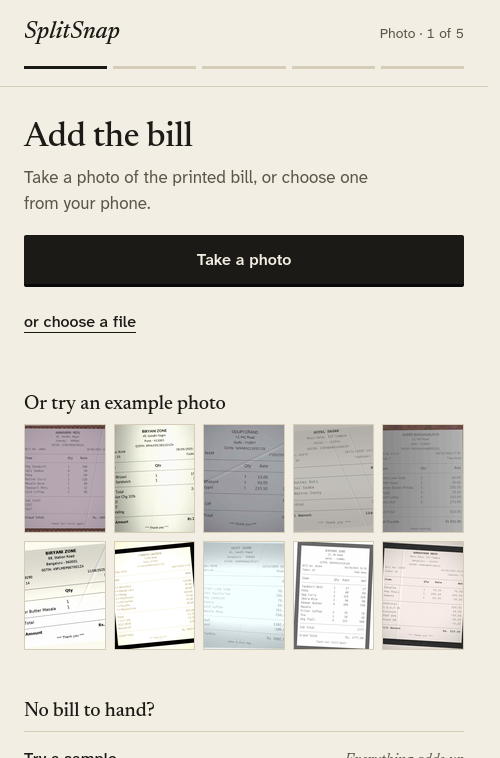
\includegraphics[width=0.185\textwidth]{figs/ui_phone_1_photo.png} &
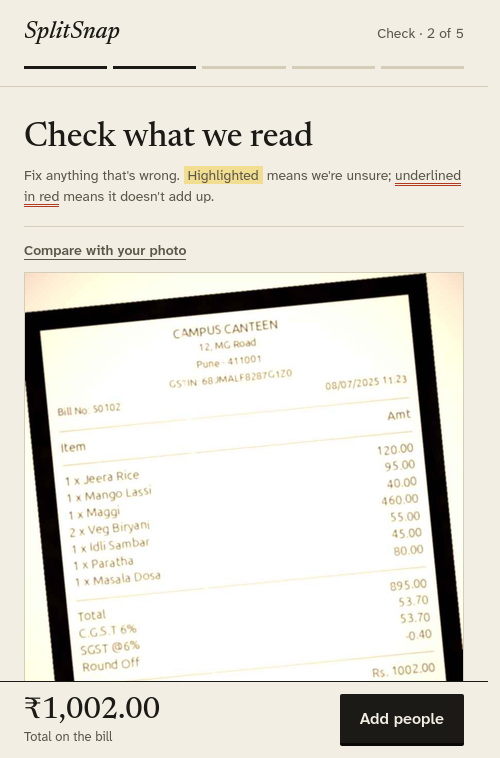
\includegraphics[width=0.185\textwidth]{figs/ui_phone_2_check.png} &
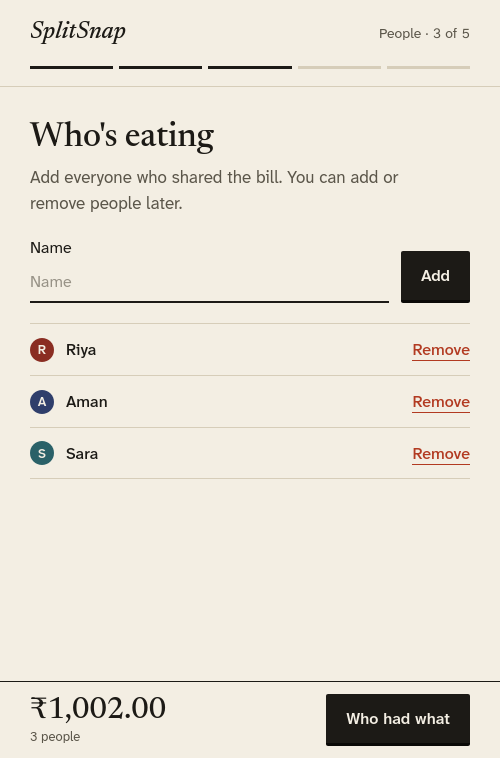
\includegraphics[width=0.185\textwidth]{figs/ui_phone_3_people.png} &
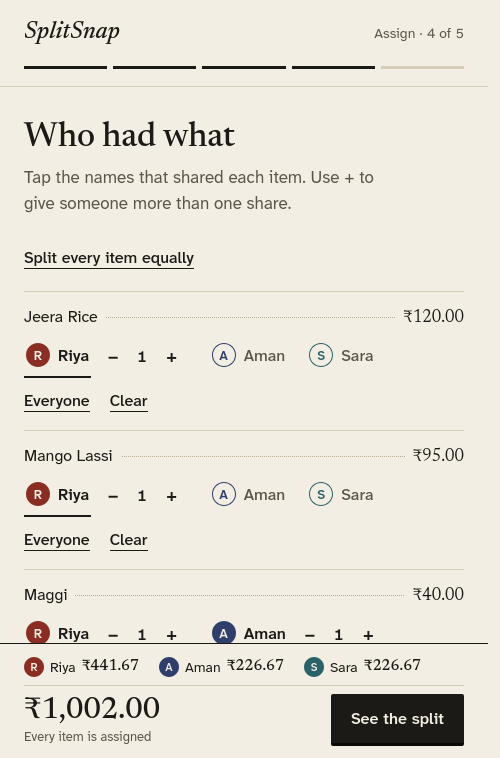
\includegraphics[width=0.185\textwidth]{figs/ui_phone_4_assign.png} &
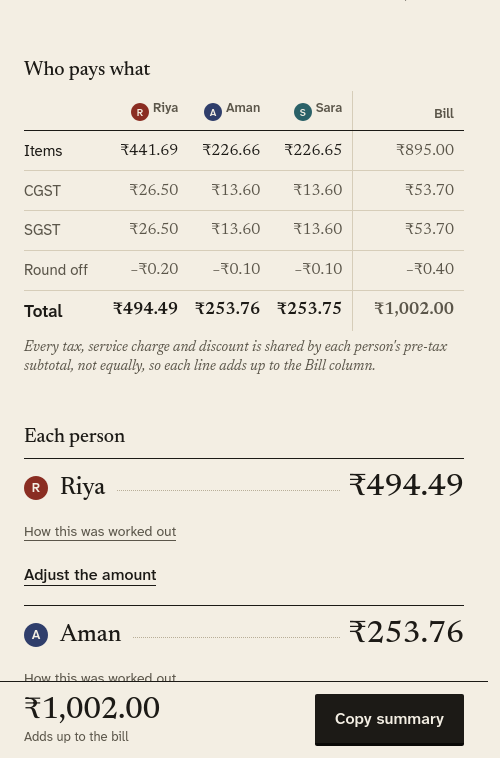
\includegraphics[width=0.185\textwidth]{figs/ui_phone_5_matrix.png}\\[1pt]
\scriptsize 1 Photo & \scriptsize 2 Check & \scriptsize 3 People & \scriptsize 4 Assign & \scriptsize 5 Split
\end{tabular}
\caption{The five steps on a phone-sized screen, reading a generated bill with the real model: photo, check (photo expanded), people, assignment, and the split with each charge divided per person.}\label{fig:ui}
\end{figure}

\begin{figure}[!ht]
\centering
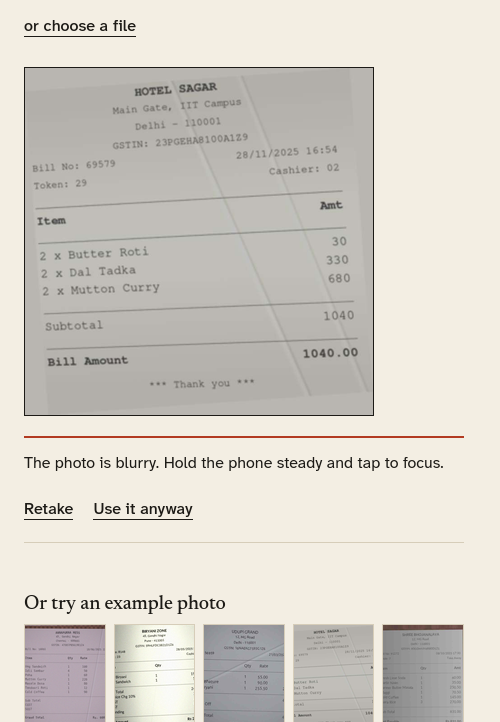
\includegraphics[width=0.30\textwidth]{figs/ui_phone_retake.png}\hspace{8mm}
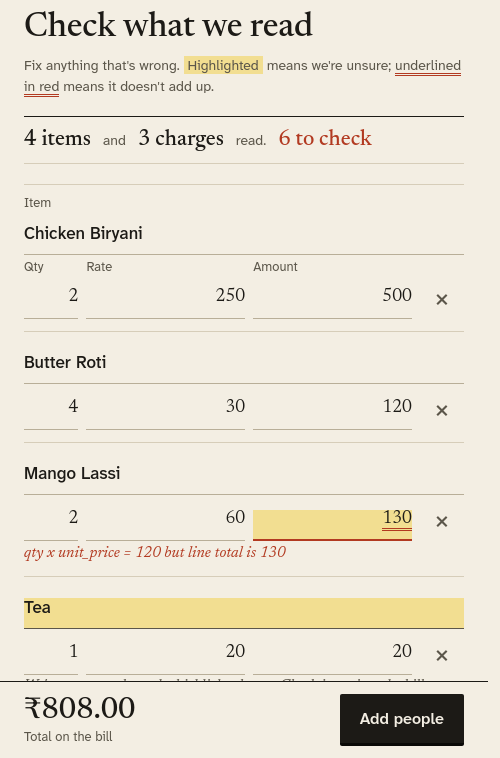
\includegraphics[width=0.30\textwidth]{figs/ui_phone_messy.png}
\caption{Confidence-driven behaviour. Left: a faded, blurred photo makes the app ask for a retake before reading, with a way to continue anyway. Right: on the correction screen a low-confidence field is highlighted in yellow, and a line whose quantity times price does not equal its total is underlined in red with the arithmetic spelled out.}\label{fig:r2}
\end{figure}

\begin{figure}[!ht]
\centering
\figimg{width=0.53\textwidth}{figs/ui_wide_2_check.png}\hfill
\figimg{width=0.44\textwidth}{figs/ui_wide_5_matrix.png}
\caption{Wide layout: the photo beside the fields on the check step (left) and the per-person charge table on the split step (right).}\label{fig:wide}
\end{figure}

\clearpage
\subsection{Two of the three processed sample bills}
These bills are among the 100 unseen generated bills; all three processed sample bills, with every intermediate file, are in \texttt{examples/processed\_bills/}. For each, the real model read the photo through the app; the corrections listed are the ones a user would make on the check screen (here, wherever the reading differed from the label); three people then shared the bill and the app produced the amounts and the explanation, shown for Sara.

\needspace{8.2cm}\noindent\begin{minipage}[t]{3.1cm}\vspace{0pt}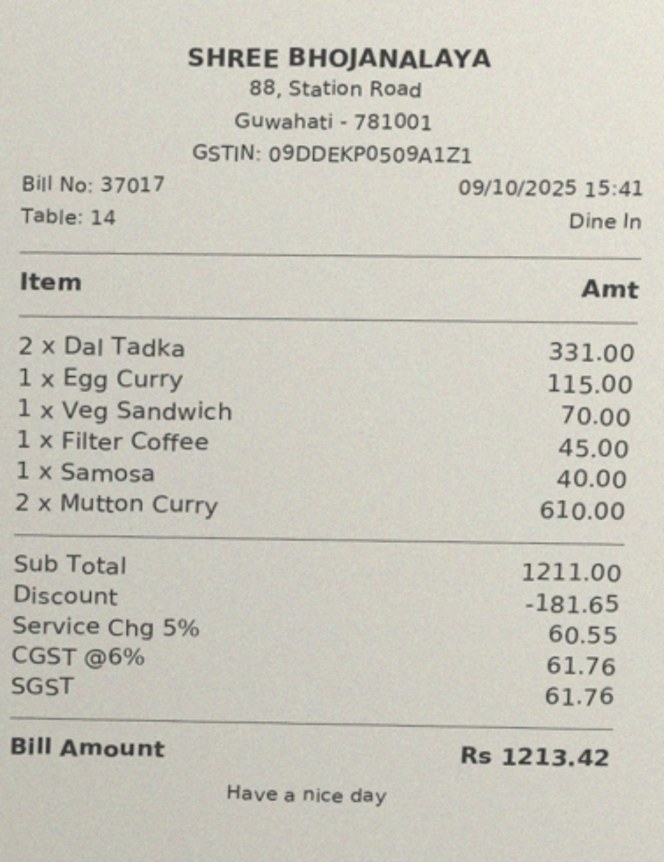
\includegraphics[width=3.1cm]{../examples/final_run/final_001.jpg}\end{minipage}\hfill
\begin{minipage}[t]{\dimexpr\linewidth-3.4cm\relax}\vspace{0pt}{\footnotesize\renewcommand{\arraystretch}{1.0}
\textbf{Bill 1.} The model read 6 items and 4 charges. Corrections made on the check screen: Mutton Curry: unit price read 310, corrected to 305.\\[2pt]
\begin{tabular}{@{}lrrrr@{}}\toprule & Riya & Aman & Sara & Bill\\\midrule
Dal Tadka & 110.34 & 110.33 & 110.33 & 331.00 \\
Egg Curry & 76.67 & 38.33 & 0.00 & 115.00 \\
Veg Sandwich & 0.00 & 0.00 & 70.00 & 70.00 \\
Filter Coffee & 45.00 & 0.00 & 0.00 & 45.00 \\
Samosa & 0.00 & 40.00 & 0.00 & 40.00 \\
Mutton Curry & 0.00 & 305.00 & 305.00 & 610.00 \\
\midrule
Discount & $-$34.80 & $-$74.05 & $-$72.80 & $-$181.65 \\
Service Charge & 11.60 & 24.68 & 24.27 & 60.55 \\
CGST & 11.83 & 25.18 & 24.75 & 61.76 \\
SGST & 11.83 & 25.18 & 24.75 & 61.76 \\
\midrule
Total (Rs) & \textbf{232.47} & \textbf{494.65} & \textbf{486.30} & \textbf{1213.42} \\
\bottomrule\end{tabular}\\[2pt]
\textit{Sara: Dal Tadka (1/3 share, Rs 110.33) + Veg Sandwich (full, Rs 70.00) + Mutton Curry (1/2 share, Rs 305.00) = Rs 485.33 pre-tax subtotal. Sara's pre-tax subtotal is 40.1\% of the Rs 1211.00 of items on the bill, so Sara carries 40.1\% of each tax, service charge, discount and rounding line. ...}}\end{minipage}
\par\vspace{5pt}

\needspace{8.2cm}\noindent\begin{minipage}[t]{3.1cm}\vspace{0pt}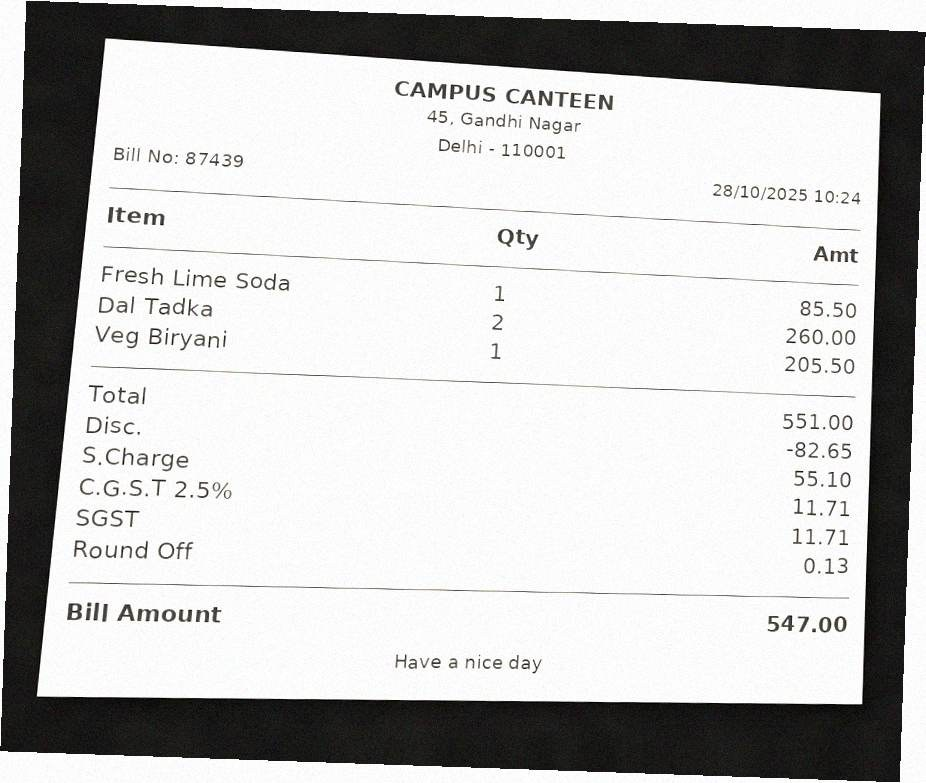
\includegraphics[width=3.1cm]{../examples/final_run/final_016.jpg}\end{minipage}\hfill
\begin{minipage}[t]{\dimexpr\linewidth-3.4cm\relax}\vspace{0pt}{\footnotesize\renewcommand{\arraystretch}{1.0}
\textbf{Bill 2.} The model read 3 items and 5 charges. Corrections made on the check screen: none needed.\\[2pt]
\begin{tabular}{@{}lrrrr@{}}\toprule & Riya & Aman & Sara & Bill\\\midrule
Fresh Lime Soda & 28.50 & 28.50 & 28.50 & 85.50 \\
Dal Tadka & 173.33 & 86.67 & 0.00 & 260.00 \\
Veg Biryani & 0.00 & 102.75 & 102.75 & 205.50 \\
\midrule
Discount & $-$30.27 & $-$32.69 & $-$19.69 & $-$82.65 \\
Service Charge & 20.18 & 21.79 & 13.13 & 55.10 \\
CGST & 4.29 & 4.63 & 2.79 & 11.71 \\
SGST & 4.29 & 4.63 & 2.79 & 11.71 \\
Round Off & 0.05 & 0.05 & 0.03 & 0.13 \\
\midrule
Total (Rs) & \textbf{200.37} & \textbf{216.33} & \textbf{130.30} & \textbf{547.00} \\
\bottomrule\end{tabular}\\[2pt]
\textit{Sara: Fresh Lime Soda (1/3 share, Rs 28.50) + Veg Biryani (1/2 share, Rs 102.75) = Rs 131.25 pre-tax subtotal. Sara's pre-tax subtotal is 23.8\% of the Rs 551.00 of items on the bill, so Sara carries 23.8\% of each tax, service charge, discount and rounding line. ...}}\end{minipage}
\par\vspace{5pt}


\clearpage
\section{Optimisation, latency and serving}\label{sec:opt}
\small
\textbf{Where the time goes.} One bill at a time, greedy decoding, at most 512 tokens, on a laptop RTX 4050 (median of 20 images: scans, generated bills and phone-size photos). Preparation is CPU work (decode, resize); the encoder is one pass; the decoder writes the answer token by token and is the largest part, which is why long bills take longer.

\begin{figure}[!ht]
\centering
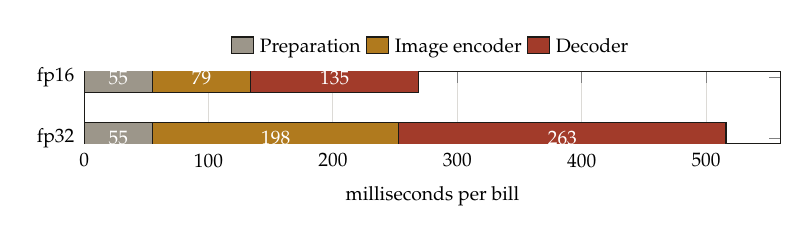
\begin{tikzpicture}
\begin{axis}[xbar stacked,width=0.86\textwidth,height=2.5cm,bar width=11pt,symbolic y coords={fp32,fp16},ytick=data,xlabel={milliseconds per bill},xmin=0,xmax=560,legend style={at={(0.5,1.04)},anchor=south,legend columns=3},nodes near coords,every node near coord/.append style={font=\scriptsize,text=white},xmajorgrids]
\addplot[fill=ash,draw=ink] coordinates {(55,fp32) (55,fp16)};
\addplot[fill=ochre,draw=ink] coordinates {(198,fp32) (79,fp16)};
\addplot[fill=brick,draw=ink] coordinates {(263,fp32) (135,fp16)};
\legend{Preparation,Image encoder,Decoder}
\end{axis}
\end{tikzpicture}
\end{figure}

\textbf{What we changed for inference.}
\begin{table}[!ht]
\centering\footnotesize
\begin{tabular}{@{}p{4.6cm}p{9.2cm}l@{}}
\toprule
Change & Measured effect & Status\\
\midrule
Half precision (fp16) & median 538 to 285 ms (1.9$\times$ faster), p95 979 to 505 ms, GPU memory 1.43 to 0.72 GB, identical output on 20 of 20 images & in use\\
Load and warm the model at start-up & first request 626 ms against about 245 ms afterwards, so the first user no longer waits an extra 380 ms & in use\\
fp16 checkpoint file & 809 MB to 411 MB, same answers (20/20), same speed & in use\\
Cheaper JPEG decode for large photos & 12-megapixel photo: request 426 to 261 ms ($-$39\%); no effect on small images; one field in about 120 changed in our tests & opt-in\\
\texttt{torch.compile} on the encoder & 437 to 373 ms ($-$15\%), identical output on 4 of 4 bills, 30 s compile on first call & not enabled\\
\bottomrule
\end{tabular}
\end{table}

\textbf{Tried and not adopted.} Compiling the decoder as well as the encoder (426 ms) and removing the unknown-token filter (288 against 285 ms) gave nothing. int8 weight-only quantisation (torchao) was slower (338 ms for the decoder, 367 ms for the whole model, against 264 ms for fp16) and changed the answers on most of 12 bills; FP8 was 2.7 to 3.4 times slower. The model is already only 0.72 GB in fp16, and at one bill at a time the extra conversion work costs more than it saves, so we kept fp16.

\textbf{Training.} A 24-step benchmark on the T4 (batch 1, fp16) chose the configuration: dropping gradient checkpointing took a sample from 0.58 s to 0.46 s ($-$21\%) and still fits (7.2 GB); 8-bit AdamW saved memory but not time. The real run reached 0.42 s per sample. Dynamic target padding, a 512-token limit, fused AdamW, pinned memory, persistent loader workers and a 2,560-pixel cap on image size (some SROIE scans are 35 megapixels) are also in use; we did not time each of those on its own.

\textbf{Serving capacity.} We sent concurrent uploads of unique photos to the running app (the model runs in a worker thread, one bill on the GPU at a time) while probing a light endpoint (``Validate'', the live bill check). Measured on the laptop GPU:
\begin{center}\begin{tabular}{@{}rrrrrrr@{}}
\toprule
Clients at once & Requests & Bills per s & Latency p50 (s) & Latency p95 (s) & Validate p50 (ms) & Validate max (ms)\\
\midrule
1 & 5 & 2.85 & 0.33 & 0.47 & 1 & 2 \\
2 & 10 & 2.78 & 0.71 & 0.85 & 1 & 3 \\
4 & 20 & 2.79 & 1.43 & 1.83 & 1 & 2 \\
8 & 40 & 2.80 & 2.83 & 3.52 & 1 & 14 \\
\bottomrule
\end{tabular}
\end{center}
Throughput stays at about 2.8 bills per second however many people ask at once, and the wait grows with the queue (median 0.33 s alone, 2.83 s with eight at once), while the light endpoint stays under 14 ms, so editing and splitting are not held up by someone else's photo. Capacity therefore comes from adding GPUs. The estimate below is arithmetic on the measured latency, not a deployed test: 0.5 s of GPU time per bill (the T4 median was 0.455 s), a peak of three times the hourly average, and a target of 60\% GPU use.
\begin{center}\footnotesize
\begin{tabular}{@{}rrrp{6.2cm}@{}}
\toprule
Bills read per hour & Peak bills per s & T4 GPUs (estimate) & Note\\
\midrule
100 & 0.08 & 1 & idle most of the time\\
1,000 & 0.83 & 1 & about 70\% of one GPU at the peak\\
10,000 & 8.3 & 7 & \\
100,000 & 83 & 70 & needs batching or a smaller model to be affordable\\
\bottomrule
\end{tabular}
\end{center}
A model copy needs about 0.72 GB of GPU memory, so memory is not the limit, and CPU preparation is 55 ms per bill, so a few cores per GPU are enough. Batching bills, larger GPUs and CPU-only serving are untested.
\normalsize


\clearpage
\section{Limitations and future work}\label{sec:limits}
\textbf{No photographed Indian bills.} The problem statement asks for generalisation to real Indian restaurant and canteen bills, and we did not have a labelled set of them. Everything we report about Indian-style layouts (charge lines, GST wording, rupee formats) is measured on bills our own generator draws, both the 100-bill test split and the 100 further bills used for the before and after comparison. Those scores show that the model has learned the output format and the charge vocabulary, and nothing more; they cannot tell how it reads a crumpled, folded or handwritten bill from a real mess. SROIE has no item labels, so the main task never saw that kind of image: on 8 real SROIE scans, with or without six image enhancements, it returned no items at all (it wrote the four SROIE fields instead, which the auxiliary task reads well: date 8 of 8, company 7, total 7, address 4). The app now uses that auxiliary reading to offer the shop name and total and asks for the items by hand. Whether real restaurant bills behave like these retail scans or like CORD's restaurant photos is exactly what real Indian bills would tell us.

\textbf{Evaluation caveats.} The metrics are our own implementation, not an official scorer. The EDA found many near-duplicate image pairs across the CORD and SROIE splits (likely the same shop's template), which we did not check by eye, so the held-out scores may be slightly generous. About 15\% of CORD labels do not satisfy their own arithmetic, which caps the arithmetic-consistency score and the CORD charge F1. The confidence analysis uses CORD and generated validation bills only; SROIE fields have no confidence. The checkpoint was selected on validation bills, so validation scores are a little optimistic compared with the test scores (CORD edit-distance score 0.958 against 0.930). The zero-shot comparison of larger models is not a comparison after training.

\textbf{Serving.} The reference app has no sign-in, rate limit or persistent storage, handles one bill per GPU at a time, and was load-tested on a single laptop GPU, not on a deployed server.

\subsection*{Future work}
\begin{itemize}
\item \textbf{Real bills.} Collect and label 60--150 photographed Indian bills, evaluate on at least 30 held-out ones, and fine-tune with the rest; this is the largest gap in the evidence.
\item \textbf{Running on the phone.} The fp16 model is 411 MB, too large to ship comfortably inside an app. Options are exporting the encoder and decoder to a mobile runtime (ONNX Runtime Mobile, Core ML, TensorFlow Lite), distilling into a smaller student, lowering the input resolution after measuring the accuracy cost, and quantising with a mobile toolchain. Our int8 and FP8 tests were run in eager PyTorch on a desktop GPU and do not predict how an NPU kernel behaves, so each of these needs its own accuracy check before it is trusted. A hybrid is also possible: a phone does capture and quality checks and the server reads the bill.
\item \textbf{Tilt and the retake prompt.} Extend the straightening estimator beyond 10 degrees and check it on real photos; retune the retake thresholds, which were set on CORD and SROIE photos and are over-cautious on our generated bills.
\item \textbf{Faster serving.} TensorRT or ONNX export of the encoder, a static key-value cache for the decoder, batching of concurrent requests, and a decision on whether to enable the compiled encoder after a larger test.
\item \textbf{Harder bills.} Hindi and other scripts, handwritten totals, bills longer than one photo (stitching several photos), partial-occlusion augmentation, and a fine-tuned vision-language model (for example a LoRA-trained Qwen3-VL-2B) as a challenger to compare accuracy against Donut.
\item \textbf{Product.} Saved groups, payment links, and an offline-capable installable web app.
\end{itemize}

\subsection*{Open-source compliance and reproducibility}
No closed or paid model or API is called anywhere in the extraction pipeline or the app; inference needs no network access. The base model, libraries, fonts and the CORD and SROIE data are open or publicly available, and \texttt{OPEN\_SOURCE.md} lists each component. Training code (\texttt{splitsnap/train.py} and the Kaggle runner), the split manifest builder, the evaluation scripts and the logs behind every figure in this report are in the repository.


\end{document}
